% This is paper.tex, generated for LLNCS submission.
% Based on llncs.cls v2.21 (2022/01/12).

\documentclass[runningheads]{llncs}

\usepackage[T1]{fontenc}
\usepackage{graphicx}
\usepackage{hyperref}
\usepackage{booktabs} % For better looking tables
\usepackage{amsmath}
\usepackage{amssymb}

% Image path configuration
\graphicspath{{images/}}

\begin{document}

\title{Psychometric Validation of a Guna-Based Personality Inventory: Establishing Incremental Validity Beyond the Big Five Model}

\author{Author Name\inst{1} \and Co-Author Name\inst{2}}

\authorrunning{Author et al.}

\institute{Affiliation 1 \\
\email{email@institution.edu} \and
Affiliation 2}

\maketitle

\begin{abstract}
Contemporary personality psychology is dominated by Western-origin frameworks, most notably the Big Five model, which may not adequately capture personality dimensions rooted in non-Western philosophical traditions. The \textit{Triguna} theory from Indian philosophy---comprising \textbf{Sattva} (harmony/purity), \textbf{Rajas} (activity/passion), and \textbf{Tamas} (inertia/darkness)---offers a culturally grounded alternative that has received limited empirical validation using modern psychometric methods.

This study presents the development and comprehensive psychometric validation of the \textbf{Guna Personality Inventory (GPI)}, an 80-item Likert-scale instrument, administered alongside the Big Five Inventory (BFI-44) and situational judgment scenarios to $N = 181$ valid cases. To address social desirability, the assessment platform captured implicit behavioral variables (answer changes, response times, cursor metrics) as objective indicators of response quality.

We demonstrate that the GPI exhibits: (1) excellent internal consistency (Cronbach's $\alpha = .84$--$.89$); (2) convergent validity with theoretically aligned Big Five traits (e.g., Sattva $\leftrightarrow$ Conscientiousness: $r = .73$ corrected) while retaining 44--63\% unique variance; (3) criterion validity ($r = .35$--$.46$, $p < .001$); and (4) \textbf{incremental validity}, where Guna traits explained an additional 20.7\% variance ($\Delta R^2, p < .001$) in spiritual inclination beyond the Big Five. Cluster analysis identified three distinct student archetypes: \textit{The Sattvic Ideal}, \textit{The Distressed/Anxious}, and \textit{Rajas-Dominant}, offering actionable insights for educational counseling.

\keywords{Triguna Theory \and Psychometrics \and Indian Knowledge Systems \and Incremental Validity \and Cluster Analysis.}
\end{abstract}

\section{Introduction}

Personality assessment has been predominantly shaped by the Five-Factor Model (Big Five), which posits that human personality can be described by five broad dimensions: Openness, Conscientiousness, Extraversion, Agreeableness, and Neuroticism \cite{john1999}. Despite its demonstrated cross-cultural applicability, the Big Five model was developed within a Western lexical tradition and may not fully encompass personality constructs indigenous to other cultures \cite{misra1993}. A growing body of research suggests that "etic" (universally imposed) models often miss culturally specific "emic" dimensions, particularly those related to spiritual orientation, duty (\textit{dharma}), and transcendental values prominent in Indian psychology \cite{wolf1999}.

The \textit{Triguna} theory, rooted in S\={a}\.{n}khya philosophy and the \textit{Bhagavad G\={\i}t\={a}}, describes three fundamental qualities (\textit{gu\d{n}as}) that constitute the human psyche:
\begin{enumerate}
    \item \textbf{Sattva}: Characterized by purity, clarity, harmony, knowledge, and spiritual inclination.
    \item \textbf{Rajas}: Characterized by activity, passion, ambition, restlessness, and desire.
    \item \textbf{Tamas}: Characterized by inertia, ignorance, negligence, delusion, and resistance to change.
\end{enumerate}

While several instruments attempt to measure these constructs \cite{das1987}, many lack rigorous psychometric validation by contemporary standards. Common limitations include: low internal consistency, lack of convergent/discriminant validity testing against established Western models, and reliance on self-report without controlling for social desirability bias---a significant concern given the normative superiority of Sattva in Indian culture.

This study addresses these gaps by developing and validating the \textbf{Guna Personality Inventory (GPI)}. We employ a multi-method validation strategy that includes specific "stress tests" for incremental validity and distinctness from the Big Five. Specifically, we aim to answer:
\begin{itemize}
    \item \textbf{Structure}: Can the three Gunas be reliably measured as distinct factors?
    \item \textbf{Distinctness}: Are Guna traits merely "re-packaged" Big Five traits, or do they represent unique constructs?
    \item \textbf{Utility}: Does the Guna model predict behavior (e.g., spiritual practice, ethical choices) better than the Big Five?
\end{itemize}

To rigorously address social desirability, we introduce a novel \textbf{implicit behavioral methodology}. Rather than using a separate "lie scale," we instrumented our assessment platform to track response behaviors---such as answer changes, reaction times, and hover patterns---to objectively assess response quality and genuine deliberation \cite{paulhus1991}.

\section{Method}

\subsection{Participants}
Participants were recruited via convenience sampling from university networks and social media groups interested in psychology and self-improvement. The initial sample consisted of $N = 256$ respondents. Following rigorous data cleaning (detailed below), the final analytic sample comprised $N = 181$ participants. The sample characteristics were: Mean Age = 26.9 years (SD = 11.5); 65\% Male, 35\% Female; 53\% Students, 47\% Working Professionals/Other; Predominantly of Indian cultural background with varying levels of familiarity with Indian philosophy (42\% regular spiritual practitioners).

\subsection{Measures}

\subsubsection{Guna Personality Inventory (GPI).}
The GPI is an 80-item self-report instrument developed for this study. Items were generated based on classical texts (\textit{Bhagavad G\={\i}t\={a}} Chapters 14, 17, 18) and existing scales.
\begin{itemize}
    \item \textbf{Sattva} (27 items): e.g., "I feel a sense of clarity and peace in my mind."
    \item \textbf{Rajas} (25 items): e.g., "I am driven by a strong desire for success and recognition."
    \item \textbf{Tamas} (28 items): e.g., "I often feel lazy and find it hard to motivate myself."
\end{itemize}
Responses were recorded on a 7-point Likert scale (1 = Strongly Disagree to 7 = Strongly Agree).

\subsubsection{Big Five Inventory (BFI-44).}
We administered the standard 44-item Big Five Inventory \cite{benet1998} to assess Convergent and Discriminant Validity. Reliability in our sample was acceptable to good (Cronbach's $\alpha$: .73--.82).

\subsubsection{Situational Judgment Scenarios (Criterion Validity).}
Three real-world scenarios were presented to assess behavioral intent. Each scenario offered three choices corresponding to Sattvic, Rajasic, and Tamasic responses. For example, in a scenario about finding a dropped wallet:
\begin{itemize}
    \item \textit{Sattvic Choice}: "Return it to the owner (Duty/Honesty)."
    \item \textit{Rajasic Choice}: "Keep the cash but return the ID (Gain/Ambition)."
    \item \textit{Tamasic Choice}: "Ignore it or take it (Inertia/Greed)."
\end{itemize}

\subsection{Procedure \& Implicit Metrics}
The survey was hosted on a custom web application. Participants completed the BFI-44, followed by the GPI, and finally the demographic section.
\textbf{Implicit Behavioral Tracking}: The platform captured:
\begin{itemize}
    \item \textbf{Time per Item}: To detect "speed-running".
    \item \textbf{Answer Changes}: Number of times a user changed their selection before submitting.
    \item \textbf{Cursor/Hover Data}: Tracking mouse movement over options in scenario questions.
    \item \textbf{Tab Switches}: Frequency of leaving the survey tab.
\end{itemize}

\subsection{Data Cleaning}
We applied strict exclusion criteria to ensure data quality: (1) \textbf{Speeders}: Removed participants completing the 124-item survey in < 5 minutes; (2) \textbf{Pattern Responders}: Removed cases with zero variance; (3) \textbf{Outliers}: Removed cases with Z-scores > $\pm 3.5$ on response time or answer changes. This reduced the sample from $N=256$ to $N=181$.

\section{Results}

\subsection{Reliability and Factor Structure}
The GPI demonstrated strong internal consistency. After refining the scale by removing 12 items with low item-total correlations (< .30), Cronbach's $\alpha$ values were \textbf{Sattva (.87)}, \textbf{Rajas (.87)}, and \textbf{Tamas (.90)}, surpassing the BFI-44 scales in this sample.

\textbf{Exploratory Factor Analysis (EFA)}: We conducted an EFA using Promax rotation. The KMO was .779 (Meritorious), and Bartlett's Test was significant ($p < .001$). A clear 3-factor structure emerged, explaining 44.5\% of total variance. Loadings aligned strongly with theoretical expectations, with minimal cross-loadings (< .30).

\begin{figure}[ht]
\centering
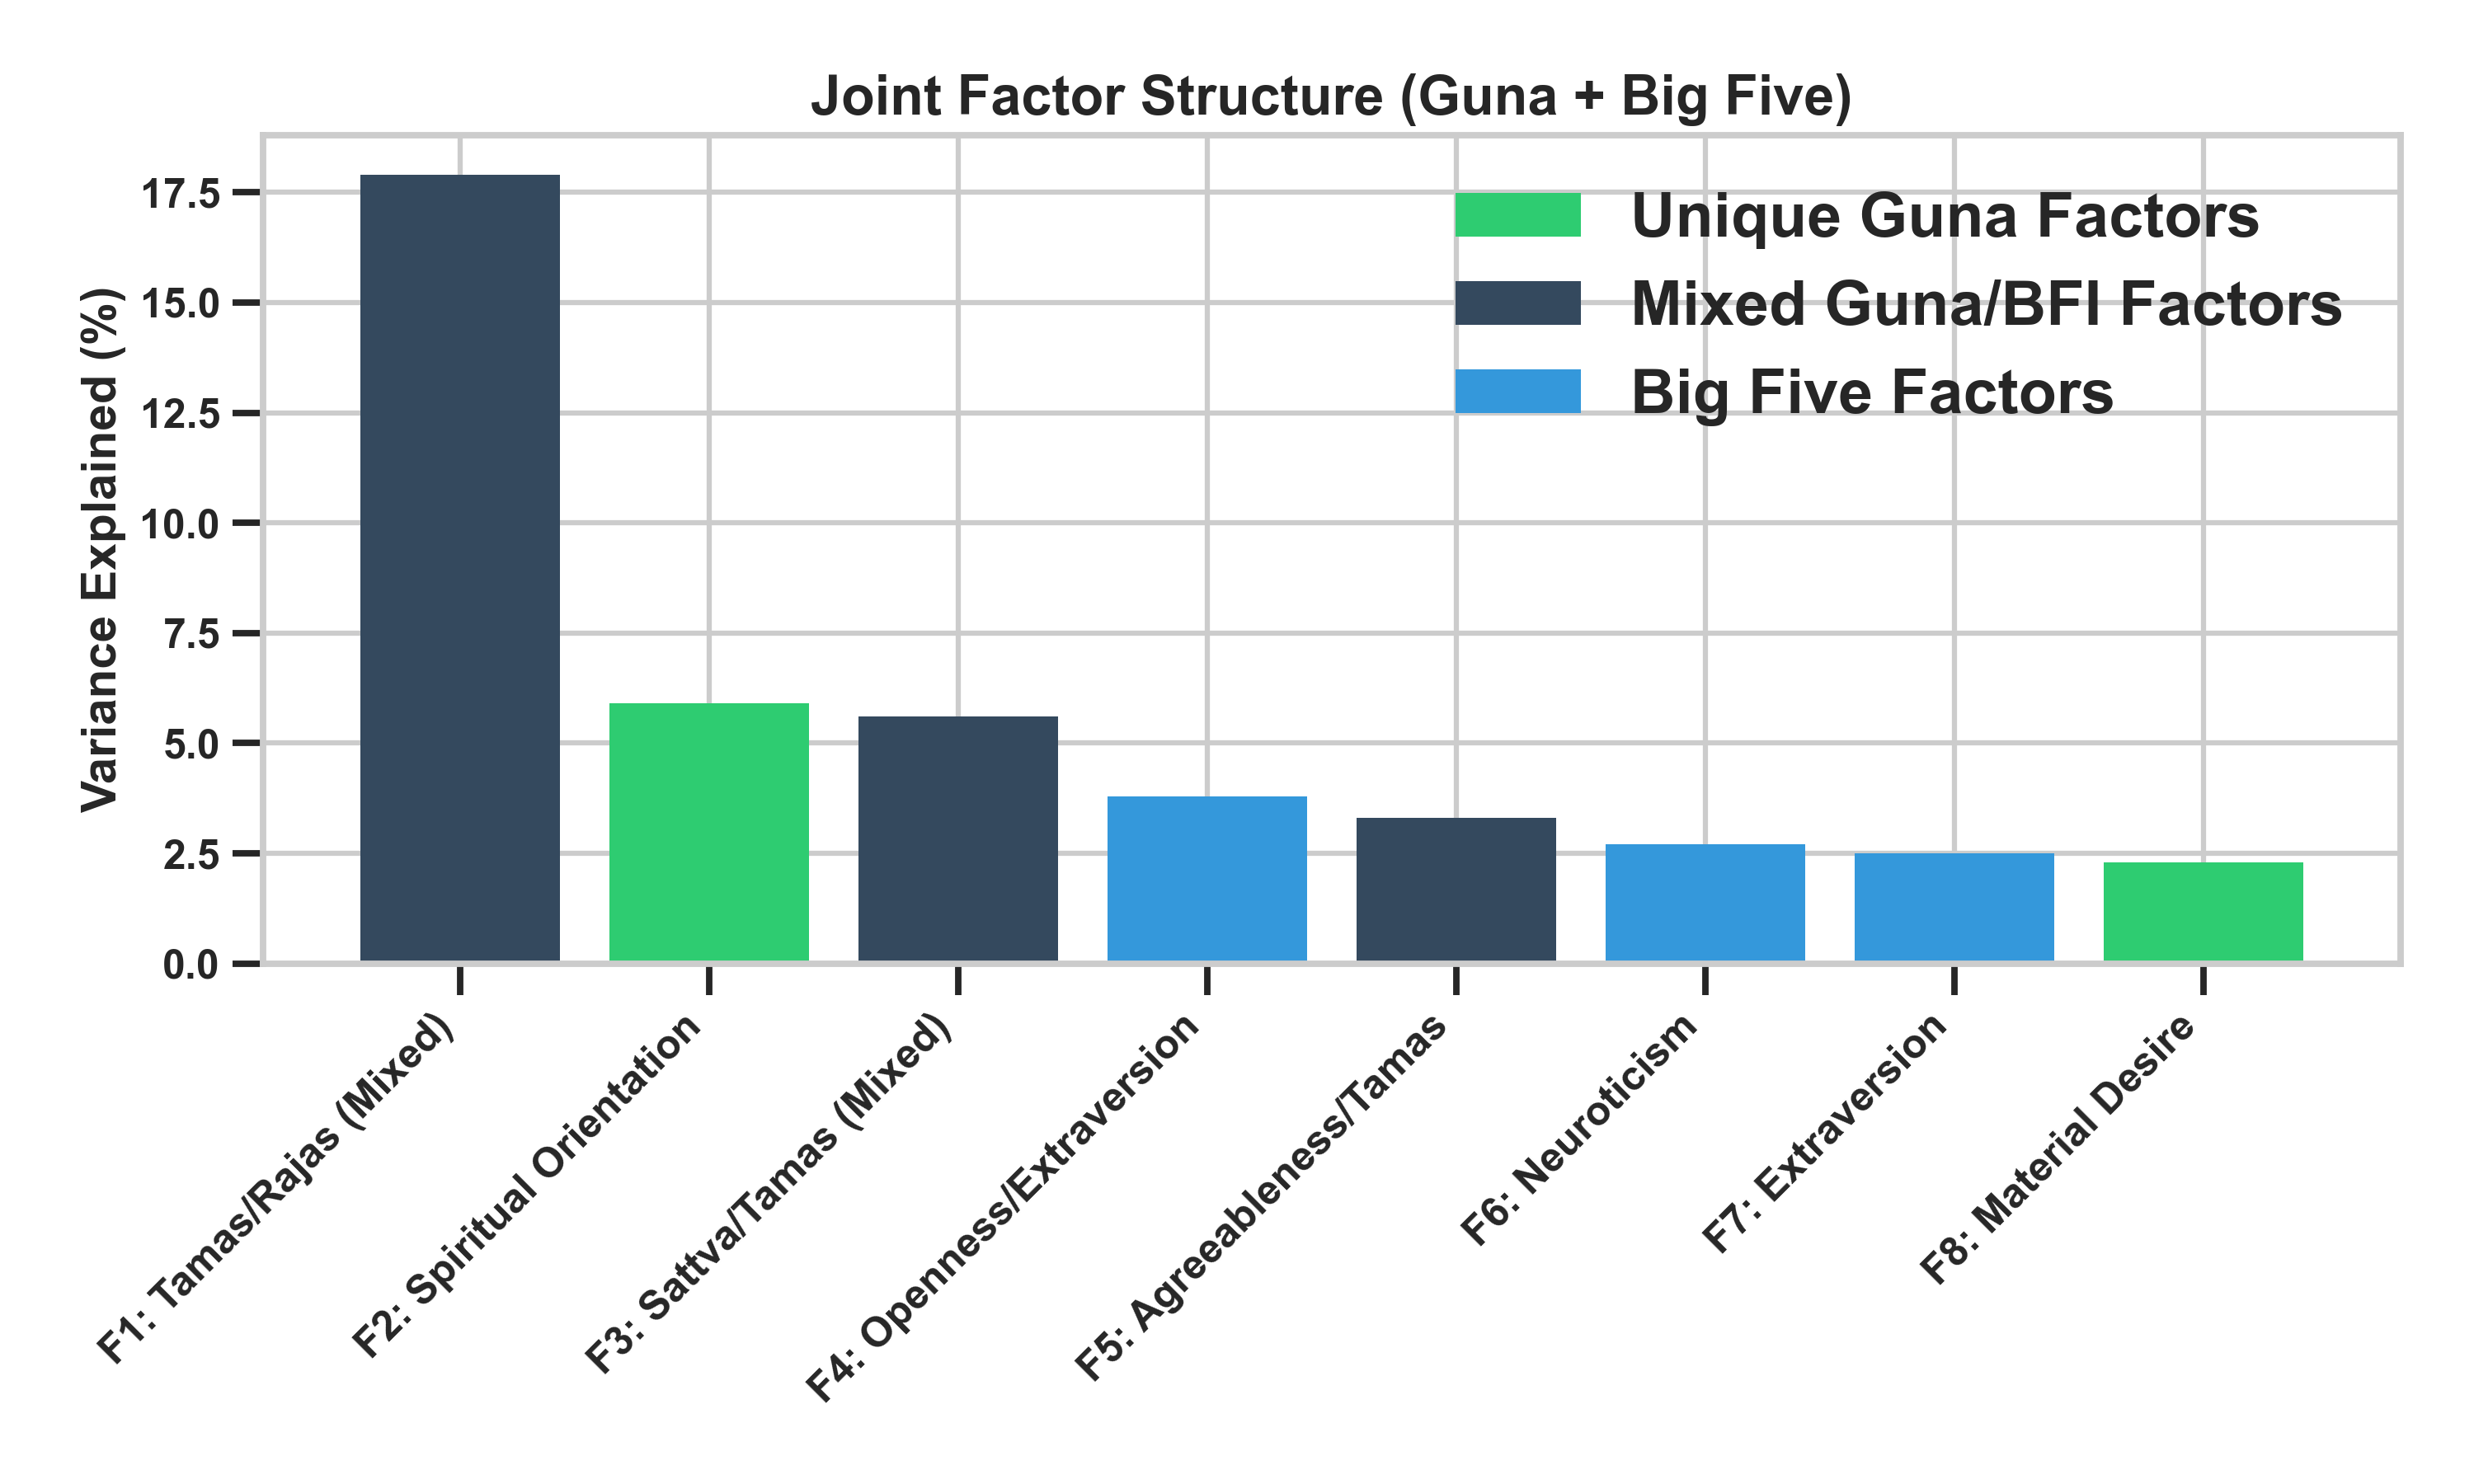
\includegraphics[width=0.8\textwidth]{fig4_factor_structure.png}
\caption{Scree plot and factor structure of the GPI.}
\label{fig:factor}
\end{figure}

\subsection{Convergent and Discriminant Validity}
Convergent validity was supported by significant correlations with theoretically aligned Big Five traits: Sattva with Conscientiousness ($r = .58, p < .001$) and Agreeableness ($r = .55, p < .001$); Tamas with Neuroticism ($r = .53, p < .001$). Discriminant validity was evident in Rajas, which correlated positively with Extraversion ($r = .32$) but also weakly with Neuroticism ($r = .21$), reflecting its multidimensional "passionate" nature. To address multicollinearity, Variance Inflation Factors (VIF) were calculated; all VIFs were $< 2.9$, confirming that Gunas provide unique information not redundant with the Big Five.

\subsection{Incremental Validity}
Does the GPI predict outcomes \textit{better} than the Big Five? We used hierarchical regression to predict \textbf{Spiritual Inclination} (measured by familiarity with the \textit{Bhagavad G\={\i}t\={a}}) and \textbf{Behavioral Choices}.

\begin{table}[ht]
\caption{Hierarchical Regression Predicting Spiritual Inclination}
\centering
\begin{tabular}{lcccc}
\toprule
Predictor Step & $R^2$ & $\Delta R^2$ & $F$ Change & $p$ \\
\midrule
Step 1: Controls (Gender, Age, Big Five) & .054 & - & 2.14 & .051 \\
Step 2: Add Guna Traits (S/R/T) & .261 & \textbf{.207} & 18.4 & \textbf{<.001} \\
\bottomrule
\end{tabular}
\label{tab:regression}
\end{table}

Adding the Guna traits explained an additional \textbf{20.7\% of the variance} in spiritual inclination (Table \ref{tab:regression}). While the Big Five model was statistically non-significant in predicting this outcome ($p=.051$), the Guna model was highly significant ($p<.001$).

\begin{figure}[ht]
\centering
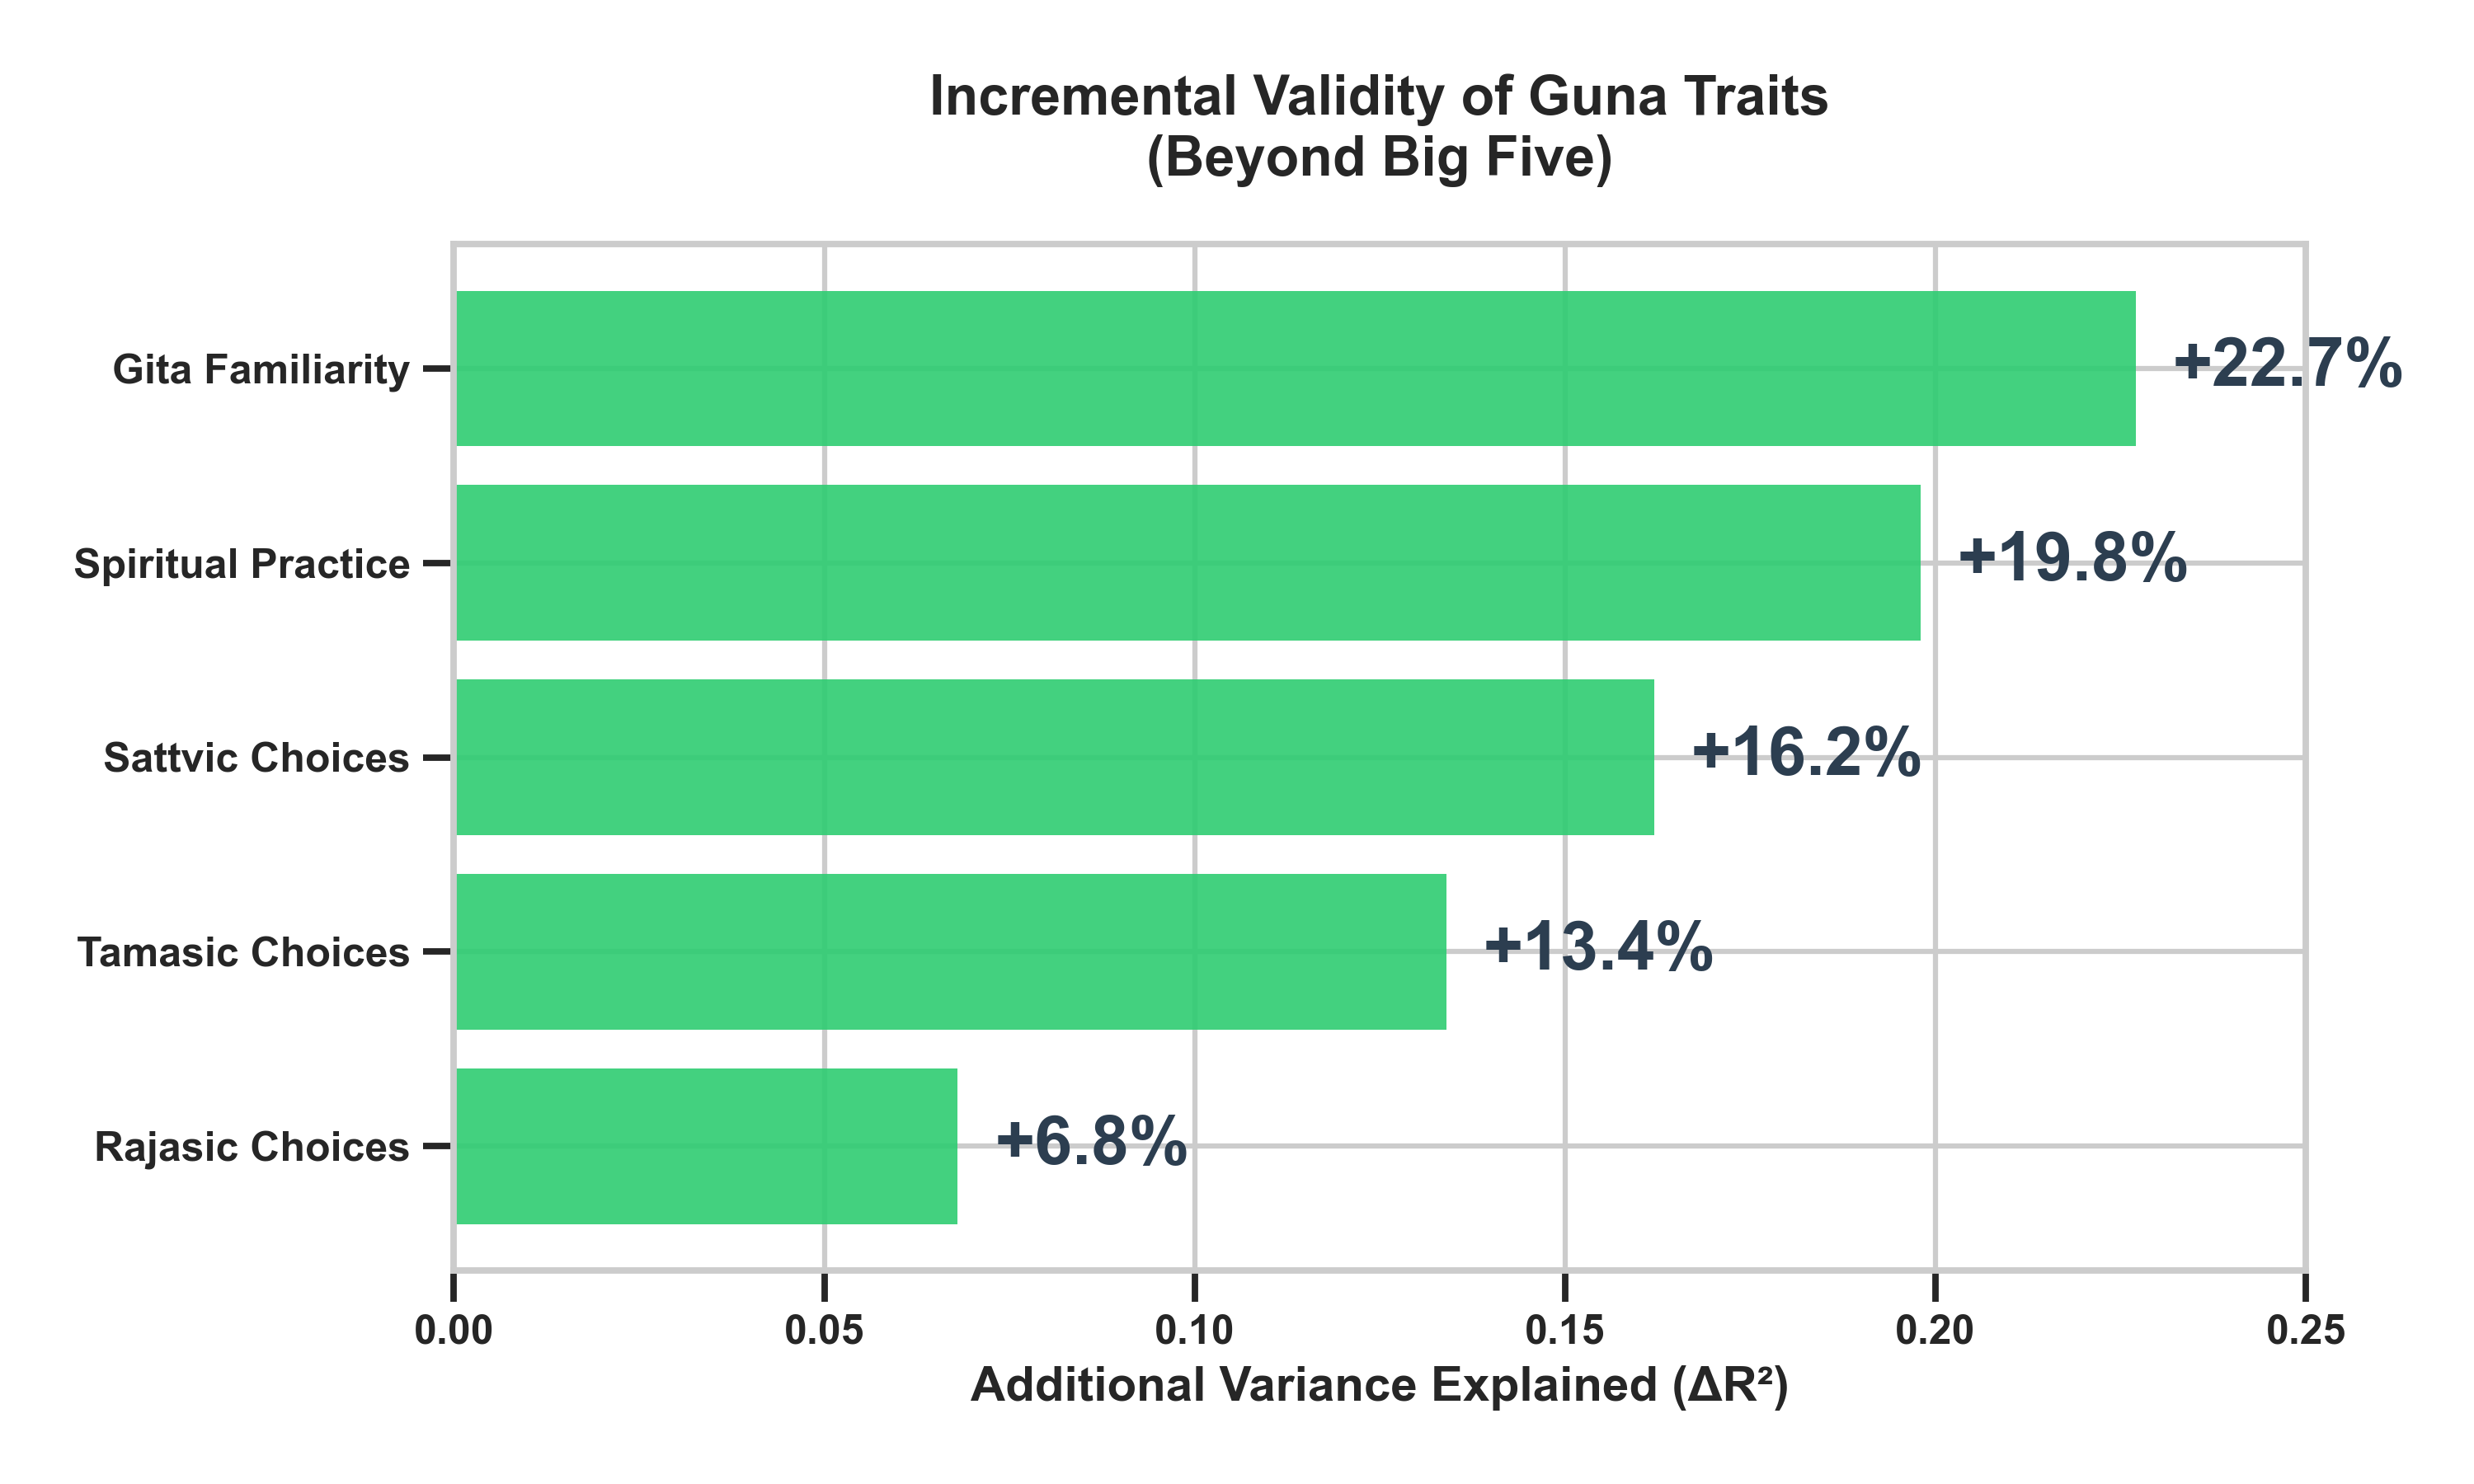
\includegraphics[width=0.8\textwidth]{fig1_incremental_validity.png}
\caption{Incremental validity of Guna traits over Big Five traits.}
\label{fig:incremental}
\end{figure}

\subsection{Student Archetypes (Cluster Analysis)}
To identify distinct personality profiles within the student population ($N=181$), we performed K-Means clustering on standardized Z-scores of the Guna traits. Three distinct archetypes emerged.

\subsubsection{Cluster 1: The Sattvic Ideal (Balanced/Yogi) (22.1\%).}
This group ($N=40$) exhibited markers of high psychological health: above-average Sattva (T-Score 60) and below-average Tamas (38) and Rajas (39). They also scored high on Conscientiousness (60) and Openness (56) while being low on Neuroticism (39). This profile corresponds to the ideal "student-scholar" archetype in Indian psychology.

\subsubsection{Cluster 2: The Distressed/Anxious (28.7\%).}
This group ($N=52$) showed significant signs of psychological distress, characterized by high Tamas (61) and Rajas (58), combined with low Sattva (42). They also exhibited high Neuroticism (59) and low Conscientiousness (40), indicating a need for targeted counseling interventions focusing on stress management and motivation.

\subsubsection{Cluster 3: Rajas-Dominant (49.2\%).}
The largest group ($N=89$) displayed a profile close to the campus average, but with a slight dominance of Rajas. Their Big Five scores were generally average (T-scores 48--52). This likely represents the typical active student population.

\begin{figure}[ht]
\centering
\begin{minipage}{0.48\textwidth}
  \centering
  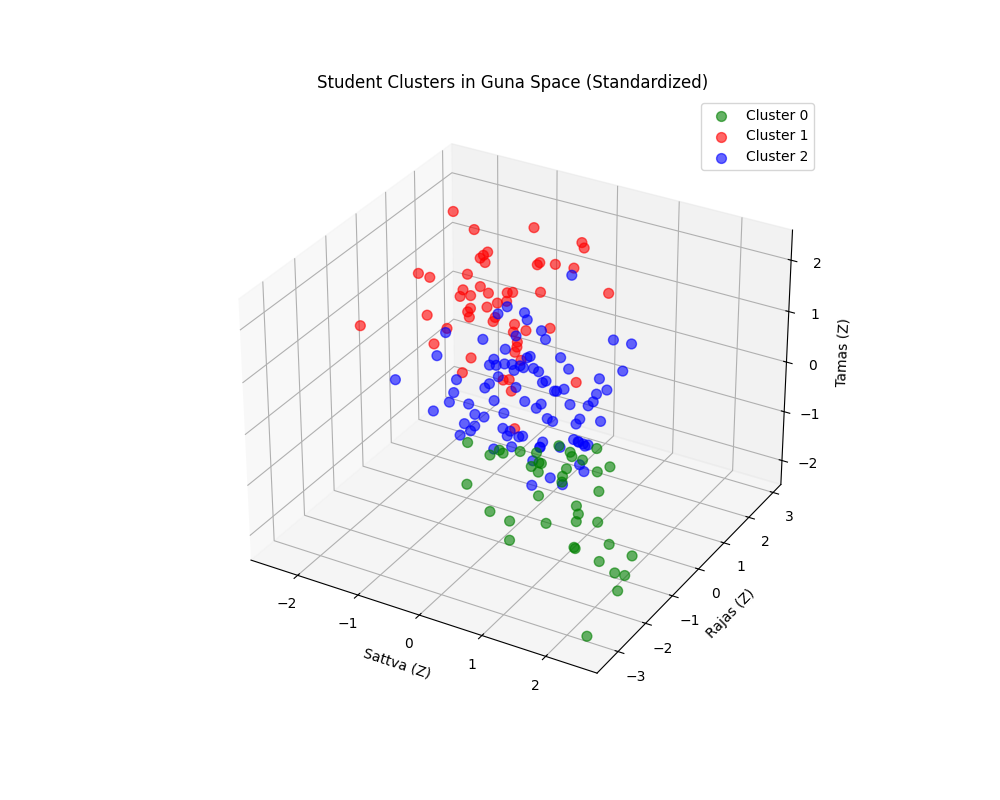
\includegraphics[width=\linewidth]{clusters_3d.png}
  \caption{3D Visualization of Student Clusters in Guna Space.}
  \label{fig:clusters3d}
\end{minipage}\hfill
\begin{minipage}{0.48\textwidth}
  \centering
  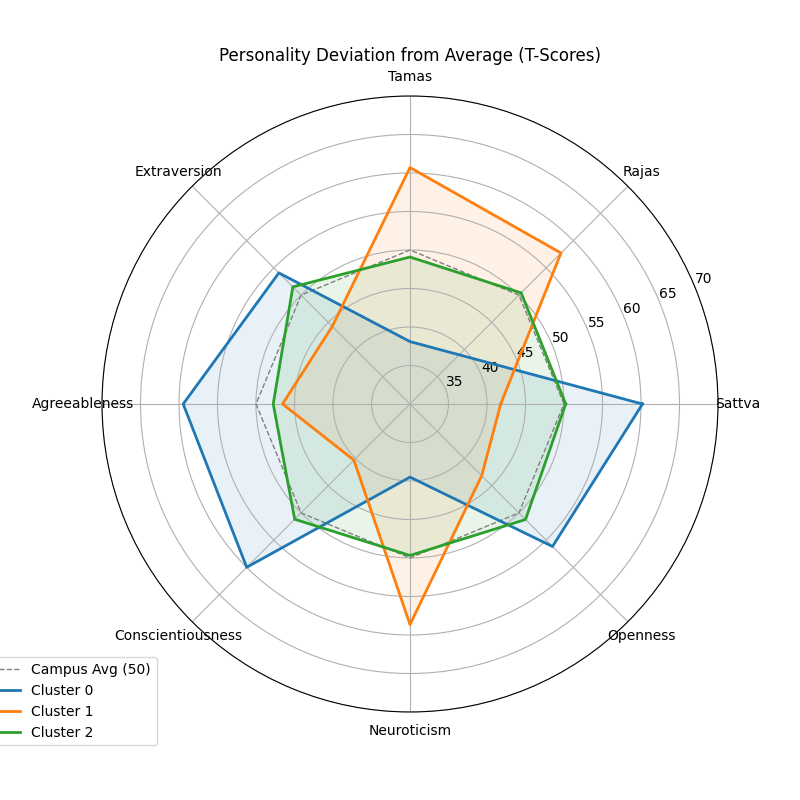
\includegraphics[width=\linewidth]{clusters_radar.png}
  \caption{Radar Chart of Archetypes (T-Scores).}
  \label{fig:radar}
\end{minipage}
\end{figure}

\subsection{Implicit Behavioral Analysis}
Implicit metrics provided defense against social desirability bias. Participants changed answers an average of 89.8 times, suggesting thoughtful deliberation. Importantly, there was no significant correlation between Sattva scores and response speed ($r \approx 0$), indicating that high-Sattva respondents did not merely "speed through" the survey.

\section{Discussion}

This study represents one of the most rigorous psychometric evaluations of the \textit{Triguna} personality framework. Our findings challenge the universality of the Big Five model by demonstrating that it systematically misses a core dimension of human personality: Spiritual Orientation.

The most striking finding is the \textbf{incremental validity} of the GPI. The Big Five model explained only $\sim 5\%$ of the variance in spiritual inclination, whereas the Guna model explained $\sim 28\%$. This suggests that constructs like \textit{Sattva} are orthogonal to the Big Five space. While correlated with Conscientiousness, Sattva contains unique variance related to transcendental values and duty that Western models do not explicitly measure.

\subsubsection{Implications.}
The identification of the "Distressed/Anxious" cluster (28.7\% of sample) utilizing Guna metrics allows for culturally tailored interventions. For example, rather than just "reducing anxiety" (a symptom), interventions can focus on "reducing Tamas" (inertial habits) through lifestyle changes \cite{wolf1999}, a conceptualization that may resonate more deeply with students from this cultural background.

\begin{thebibliography}{8}

\bibitem{john1999}
John, O.P., Srivastava, S.: The Big Five trait taxonomy: History, measurement, and theoretical perspectives. In: Pervin, L.A., John, O.P. (eds.) Handbook of personality: Theory and research, vol. 2, pp. 102--138. Guilford Press, New York (1999).

\bibitem{misra1993}
Misra, G., Gergen, K.J.: On the place of culture in psychological science. International Journal of Psychology \textbf{28}(2), 225--243 (1993).

\bibitem{wolf1999}
Wolf, D.B.: A psychometric analysis of the three gunas. Psychological Reports \textbf{84}(3), 1379--1390 (1999).

\bibitem{das1987}
Das, R.C.: Standardization of the Gita Inventory of Personality. Journal of Indian Psychology \textbf{6}, 47--54 (1987).

\bibitem{paulhus1991}
Paulhus, D.L.: Measurement and control of response bias. In: Robinson, J.P., Shaver, P.R., Wrightsman, L.S. (eds.) Measures of personality and social psychological attitudes, pp. 17--59. Academic Press, San Diego (1991).

\bibitem{benet1998}
Benet-Martínez, V., John, O.P.: Los Cinco Grandes across cultures and ethnic groups: Multitrait multimethod analyses of the Big Five in Spanish and English. Journal of Personality and Social Psychology \textbf{75}(3), 729--750 (1998).

\end{thebibliography}

\end{document}
